\chapter{绪论}
% 屏幕前的家人们你们好
% \begin{figure}[h]
%     \centering
%     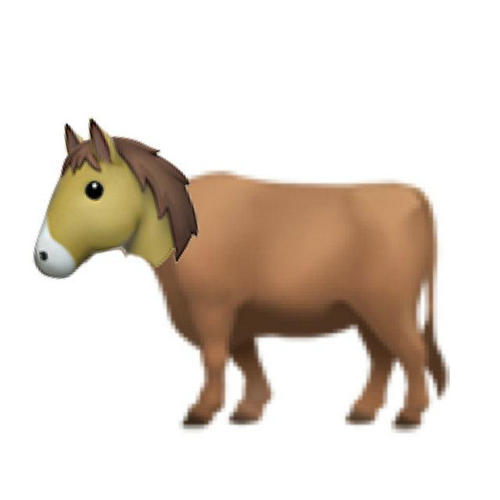
\includegraphics[width=0.5\textwidth]{figures/R-C.jpg}
%     \caption{常见的牛马形象}
%     \end{figure}
    
\section{研究背景与意义}
视觉定位作为具身智能与计算机视觉领域的核心任务，要求智能体能够通过视觉感知的方法估计相机在预先构建的环境地图中的位姿。
得益于近年来大规模且逼真的三维场景数据集的出现以及用于测试具身导航仿真器的开发，具身视觉导航在近年来取得了显著的发展。

在具身视觉导航中，一个关键问题是描述目标物体的方法。
向智能体分配任务的常见方式是下达自然语言指令，类似于“导航到目标 A ”、“到达目标 B ”等。
但当场景中相同类型的物体包含多个不同的实例时，这种分配任务的方式会产生较大的歧义，智能体常常会出现误识别或者无法识别的问题。
为解决这一歧义，Krantz等人提出了实例级目标导航 IIN \cite{krantz2022instance}。

如图\ref{fig:intro}所示，在IIN任务中，智能体接收到一张包含了特定目标物体的图像，目标是在限定时间步内找到这个特定的物体实例的位置并到达该物体附近。
这个任务要求智能体首先能够识别目标物体的具体类别，其次能够从多个不同角度来观察具有相同类别的目标物体，以确定所观察的物体实例是否与目标物体相吻合。  
\begin{figure}[htbp]
    \centering
    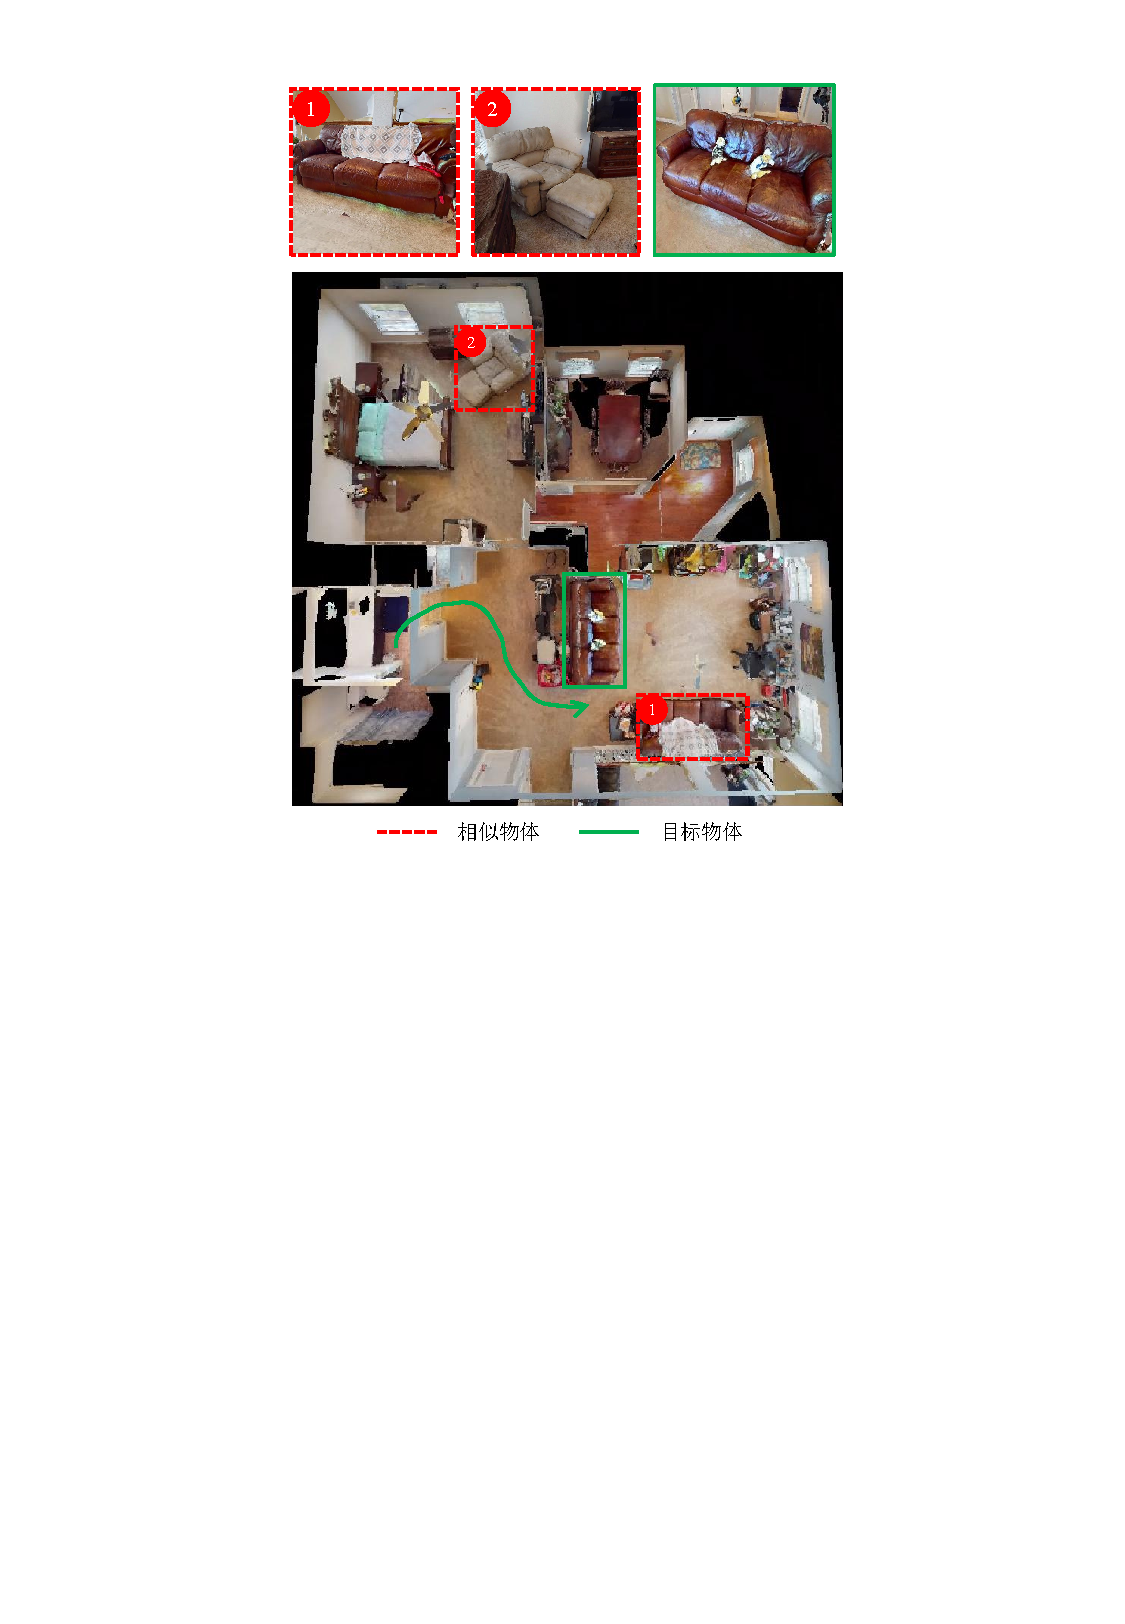
\includegraphics[width=0.7\textwidth]{figures/图标ppt/intro图片.pdf}
    \caption{实例IIN任务}
    \label{fig:intro}
\end{figure}

为解决上述的问题，现有方法所采取的策略主要是通过引入鸟瞰图（2DBEV）来处理该任务。
这种显式的地图表示方式能够大幅降低内存开销，但对于三维场景中存在的大量的物体细节，其表示能力依然受到较大局限性，所保存的语义信息和2D的几何信息对于智能体多视角观察候选目标物体这一需求支撑力有限。
此外，BEV地图也难以保存目标物体的实例级信息，而这一信息对于区分同类多个物体或者需要细粒度物体交互的任务至关重要。

为克服BEV地图局限性，Lei\cite{gaussnav}等人又针对IIN任务提出一种全新的基于3D高斯泼溅的导航框架\textbf{GaussNav}\cite{gaussnav}。
GaussNav 通过使用语义高斯地图的表示方法，将几何、语义与实例级特征的表示融为一体，得以成功应用在\textbf{边界探索、语义高斯构建、高斯导航}三阶段任务流程。
同时，Gennady Sidorov等人又针对相机位姿定位提出了\textbf{GSplatLoc}\cite{gsplatloc}——一种新颖的视觉定位框架。
该框架将基于结构的粗位姿估计与基于高斯渲染而优化的图像扭曲位姿优化策略整合到一个统一的端到端流程中，完成相机位姿估计。
这些技术在视觉导航中的目标物体描述与相机定位等具有挑战性的任务中，表现出显著的性能。

本文也基于\textbf{GaussNav}\cite{gaussnav}框架，融合了\textbf{GSplatLoc}\cite{gsplatloc}中针对高斯渲染优化后的位姿精修算法，提出了一个系统整合了几何、语义与实例级特征的地图表示的导航框架——\textbf{GSGuide}。


\section{研究现状}
本文首先简要讨论可微分渲染领域的相关研究，然后对相机定位进行全面的概述，最后在对实例级图像目标导航进行讨论。

\subsection{可微分渲染领域的相关研究}
为实现逼真的三维场景构建，早期的方法主要围绕神经辐射场（NeRF）\cite{nerf}提出。
NeRF\cite{nerf}利用单个多层感知器（MLP）来表示场景，通过沿像素光线行进并查询MLP获取不透明度和颜色值来执行体绘制。
MLP表示可以通过多视角信息优化一最小化渲染损失，从而实现高质量的新视角合成。
但NeRF\cite{nerf}的主要局限性在于训练速度较慢，且对存储需求较高，在IIN这种对于实时性要求较高的任务中，其适用性受限。

与NeRF\cite{nerf}不同的是，三维高斯溅射（3DGS）\cite{3DGS}采用可微分光栅化技术，对需要光栅化的的基元进行迭代处理，这与传统图形学中的光栅化方式类似。
利用三维场景天然的稀疏性，3DGS\cite{3DGS}能够以高保真的表示方式捕捉三维场景，同时能够显著提升渲染效率，降低存储开销。

关于三维高斯溅射技术发展的全面综述\cite{chen2024survey}强调了该方法的通用性及其在各个领域的应用。
凭借这些优势，越来越多的研究者开始探索各种创新方向，例如可变形或动态高斯\cite{luiten2024dynamic,wu20244d}、网格提取与物理模拟\cite{feng2024gaussian,xie2024physgaussian}，以及在同时定位与地图构建（SLAM）中的应用\cite{keetha2024splatam,yugay2023gaussian}。

近些年来，3DGS技术在语义增强与轻量化方向取得了重要进展，为导航任务提供了更加强大的场景表示能力。

SeG-Gaussian\cite{seg-gaussian} 提出语义引导的 3D 高斯优化框架，利用语义掩码识别重建薄弱区域，通过空间正则化抑制高斯重叠，显著提升了稀疏观测下的语义重建质量。但该方法的语义信息仅作为优化引导信号，并未嵌入高斯本身的参数表示中，无法直接支持后续的语义感知导航决策。

Gsplatloc\cite{gsplatloc} 在 3DGS 中引入原生稠密特征场，无需预训练蒸馏即可实现特征渲染，在保持实时性的同时显著提升了跨视角匹配鲁棒性。
然而其特征向量是通用视觉特征，缺乏明确的语义含义，无法直接用于目标类别过滤和实例区分，在存在多个相似物体的 IIN 任务中容易产生误匹配。

SAGE-3D\cite{sage3d} 则将 3DGS 升级为可执行、语义对齐、物理对齐的环境基础，发布了包含 1000 个室内场景的 InteriorGS\cite{sage3d} 数据集。
但该方法的语义对齐是在高斯构建完成后进行的独立后处理步骤，无法实现语义与几何参数的端到端联合优化，仍然存在语义错位问题。

鉴于高斯表示的显式特性提供了丰富的环境数据，3DGS\cite{3DGS}能够增强基于地图的视觉导航中的决策能力，可以有效地用于指导自主智能体的导航。


\subsection{相机定位领域相关研究}
视觉定位是机器人导航的核心技术，旨在估计相机相对于预构建地图的位姿。

早期的视觉重定位方法主要依赖图像检索技术，即通过查询图像与已知位姿的图像数据库进行比对来推断近似位置。
尽管这类方法计算效率高，但可扩展性较差，且对于动态环境中的定位精度会显著下降。

结构化的特征匹配方法通过利用运动恢复结构（SFM）生成的三维点云来提升定位性能。
这类方法在查询图像提取的特征与三维地图之间建立显式的2D-3D对应关系，通常结合随机抽样一致性（RANSAC）算法，使用透视$n$点（PnP）求解器来计算相机位移\cite{lim2012real}。
虽然这类方法能够实现较高的定位精度，但在处理大规模环境时，会带来巨大的内存开销。

位姿回归方法采用深度神经网络直接从输入图像估计相机位姿，大幅度降低了对大规模三维地图的依赖。
这类方法将环境结构整合到网络架构中，能够实现端到端的训练。
然而，受限于泛化能力，其性能通常不如基于结构的方法。
绝对位姿回归方法（APR）技术在计算效率和精度之间取得了一定的平衡，而场景坐标回归（SCR）通过学习紧凑的场景表示进一步提升了性能。
但场景坐标回归方法需要进行大量的优化才能达到最优精度，这限制了其在实时场景中的应用\cite{sarlin2021back}。

同样，神经辐射场\cite{nerf}和3D高斯泼溅技术\cite{3DGS}的出现，实现了高保真的新视角合成，可以在训练阶段实现数据增强，提升特征匹配能力，从而推动了视觉定位技术的发展。
基于NeRF\cite{nerf}的方法虽然有效，但往往存在推理速度慢、训练时间长以及存储开销较大的问题，在IIN\cite{krantz2022instance}这种对于实时性要求较高的任务中，其适用性受限。

% 基于3DGS的定位流程，（例如近几年的GSCPR\cite{GS-CPR}和HGSLoc\cite{hgsloc}）通常将这种三维表示用作测试时的位姿精修框架，但它们依赖外部位姿估计器来提供初始值。
随着3DGS技术的发展，基于3DGS的定位流程开始被广泛应用于IIN任务中。

GSCPR\cite{GS-CPR} GS-CPR [15] 提出基于 3D 高斯泼溅的高效相机位姿精修方法，利用 3DGS 渲染高质量参考图像和深度图，结合通用 3D 基础模型 MASt3R 建立 2D-2D 对应关系，无需训练专用特征提取器即可实现高精度位姿优化。
但该方法是纯几何的定位框架，完全不利用语义信息，无法区分同一类别的不同实例，这对于需要精确识别目标实例的 IIN 任务来说是致命的缺陷；
此外，它依赖外部的全局位姿估计器提供初始值，不具备实例级的粗定位能力，且难以满足实时导航的需求。

HGSLoc\cite{hgsloc}提出分层 3D 高斯定位框架，结合全局特征检索与局部渲染精修，有效解决了大尺度场景下的定位漂移问题。
然而其粗定位阶段采用的全局特征检索方法，对于外观相似的不同实例区分能力不足，在 IIN 任务中容易将相似物体误判为目标。

这些方法虽然在定位精度上有所提升，但均未充分考虑 IIN 任务中 "实例级区分" 的特殊需求。
本文正是针对上述问题，基于GSplatLoc\cite{gsplatloc}核心框架设计了 "语义过滤 + 细粒度特征匹配 + 渲染精修" 的三阶段定位策略，在统一的3D高斯泼溅流程中结合了基于结构的关键点匹配与基于渲染的位姿精修，利用快速可微渲染和光度扭曲损失最小化提升了定位精度。

% GS-ICP [36] 提出基于高斯的迭代最近点定位方法，将 3D 高斯的均值点作为点云进行 ICP 配准，无需渲染即可直接对齐高斯分布，在低纹理、弱光场景下鲁棒性显著提升，同时将位姿精修速度提升了 3 倍以上，为导航提供了高效无渲染的位姿精修方案。但该方法是纯几何的定位框架，完全不利用语义信息，无法区分同一类别的不同实例，且对高斯地图的几何重建质量高度敏感，当地图存在几何误差时定位精度会急剧下降，难以直接应用于需要实例级区分的 IIN 任务
\subsection{视觉导航领域相关研究}
实例级图像目标导航任务（IIN）\cite{krantz2022instance}自2022年提出以来，经历了从基于BEV地图到模块化方法到基于3DGS的新一代方法演进。
2025年，GaussNav\cite{gaussnav}提出了一种基于3DGS的模块化视觉导航框架，首次将3DGS\cite{3DGS}引入了IIN任务，取得了突破性的进展，而在此之后又有更多的研究者提出了相关工作。

UnitedVLN\cite{Unitedvln} 提出了基于通用 3D 高斯泼溅的连续视觉语言导航框架，通过统一的高斯地图表示实现了跨场景的泛化导航，在多个 VLN 基准上取得了 SOTA 性能。
该方法首次证明了 3DGS 不仅适用于单场景的实例导航，还能支持跨场景的连续长程导航任务，显著拓展了 3DGS 在具身智能领域的应用边界。
但该方法主要面向自然语言指令导航设计，其语义表示仅包含粗粒度的类别信息，缺乏对实例级细粒度特征的编码能力，无法有效区分同一类别的不同物体实例，难以直接应用于需要精确识别特定实例的 IIN 任务；
此外，其位姿估计依赖于外部 SLAM 系统，没有针对实例级目标定位进行专门优化，在存在多个相似物体的场景中容易出现定位错误。


上述工作虽然在不同方面推动了 3DGS 导航技术的发展，但仍存在两个核心局限性，也是本文工作的主要切入点：
\begin{itemize}
    \item \textbf{语义表示不充分:}大多数方法（如 GaussNav \cite{gaussnav}、UnitedVLN\cite{Unitedvln}）仍采用静态语义标签或粗粒度语义表示，无法实现语义与几何、纹理参数的端到端联合优化，导致语义错位和实例区分能力不足；
    \item \textbf{实例定位精度不足：} 现有定位方法对于相似实例的区分能力有限，且缺乏针对 IIN 任务的专用位姿精修机制，在复杂场景中容易出现目标误匹配和定位偏差。
\end{itemize}

基于此，引出本文主要工作与贡献：\textbf{基于语义增强的 3D 高斯泼溅的模块化视觉导航框架GSGuide}。



\section{本文主要工作与贡献}
本文对既有的GaussNav\cite{gaussnav}与GsplatLoc\cite{gsplatloc}两个核心框架进行了研究并进行了优化工作，提出了提出了一种基于语义增强3D 高斯泼溅的模块化视觉导航框架GSGuide。
主要贡献包括：

\begin{itemize}    
    \item \textbf{高斯语义信息融合与监督优化：} 引入Yolo26\cite{Yolo26}语义分割模型输出的物体实例语义，为高斯新增可微语义标签。复用原版3DGS中RGB颜色渲染逻辑，实现渲染通道数自适应适配RGB和语义渲染两种模式。实现了语义高斯的高效构建。
    % \item \textbf{高斯在线构建：} 使用高斯增量训练模式，并利用多线程技术在Habitat模拟器\cite{habitat-sim}中采集 Habitat-Matterport 3D (HM3D) \cite{HM3D}数据即实时使用已有数据集渲染高斯，更加贴近项目落地对于实时性要求。
    \item \textbf{对齐目标图像的具体位姿：} 利用GSplatLoc\cite{gsplatloc}提供的基于高斯渲染优化后的图像扭曲技术，通过将目标图像与高斯渲染结果进行对齐，实现了多视角生成与目标位姿精确估计。
    \item \textbf{目标导航：} 利用优化后的语义高斯表示，结合基于LightGlue+Disk\cite{lightglue,disk}的特征提取与匹配方案的目标位姿估计，实现了目标导航。
\end{itemize}

\section{论文结构安排}
本文结构安排如下：
第一章系统介绍本文的相关背景与意义；
第二章综述了三维重建、位姿对齐、视觉导航的基础理论知识；
第三章详细介绍本文工作的具体方法与实现细节；
第四章展示了在仿真环境中的实验设置、结果与分析；
第五章总结了全文工作，并对未来研究方向进行展望。